\subsection{Overview}
The basic architecture for the system is a Client-Server setup. The server will handle persistent data and contain a small subsystem for manipulating data, we will for now not describe the server or the communication between the server and client greater detail and instead focus on the client.\\

The Client-system will be made with a Model-View-Controller (MVC) architecture. The system should have different views (Log in, MonthView... etc.) which would require different event-handling. The MVC allows this because it makes it easy to do runtime changes of views and controllers. It also results in high cohesion, in that the control objects and the view objects are separated in accordance to their respective responsibilities. Both view and control objects can be separated into small classes that only handles smaller tasks. However creating the MVC-architecture requires extra code. The main architecture can be seen below (it is possible to zoom in), we have not included all views and control objects to keep things a bit clean.

\paragraph{Architecture}
\begin{center}
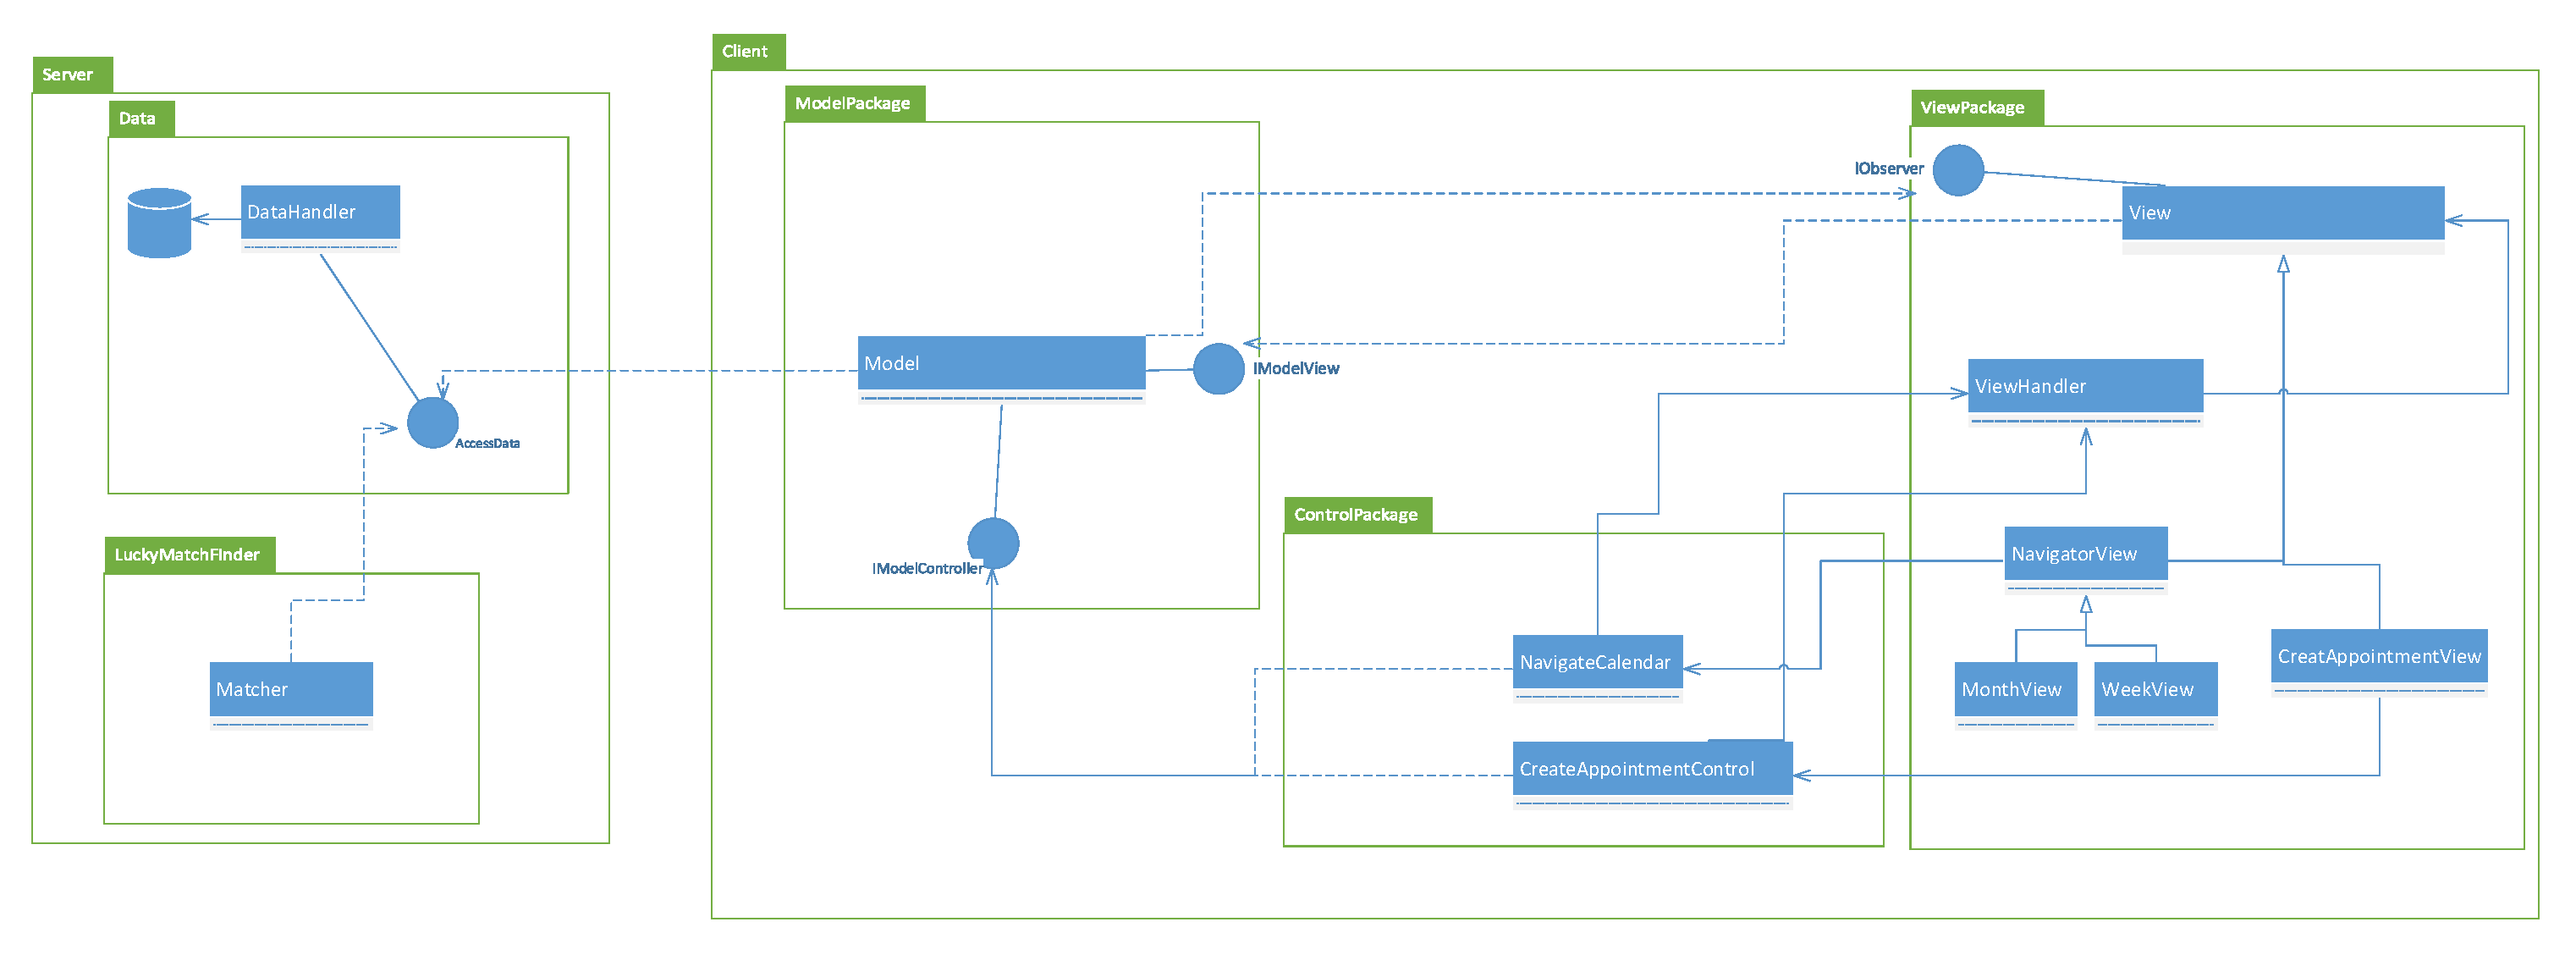
\includegraphics[scale=.4]{sections/Architecture.pdf}
\end{center}
\pagebreak

\subsection{Subsystem decomposition}
The MVC architecture gives us three distinct types of subsystems, a model that handles date, a view that handles UI, and a Control object that handles event-flow and manipulation of data. The model subsystem should function independently from the rest of the system, therefore we used a facade design pattern to hide the internal implementation of the model from the rest of the system. In addition, the model communicates with the different views through a Observer/Observable-pattern, which mean the model isn't coupled to the Views.\\

The rest of the system is divided into View and Control objects. Each View requires a Control object, that handles the event-flow of the View. Each Control object has a reference to the ViewHandler, which allows them to create a new View when necessary. \\

At this point we have identified three types of views, a NavigatorView that shows calendar navigation, a AppointmentView that shows an appointment, and a login view that allows a guest to log-in and/or create a user. Each view have one of several control objects, which handles the events caused by the user. There might be several View objects for each Control object fx. the NavigateCalender control object could be responsible for MonthView, WeekView, and DayView under the common name NavigatorView. However, the opposite is not true. One view object cannot be controlled by more than one control object. 

\subsection{Hardware/software mapping}
\subsection{Persistent data management}
\subsection{Access control and security}
\subsection{Global software control}
\subsection{Boundary conditions}
